\section{Руководство по установке и использованию} 
\label{sec:user_guide}

ПС не требует установки, достаточно собрать все компоненты и запустить их на серверах. Инструкция к сборке и запуску указана в разделе \ref{sub:creation:build_and_install}.
Все необходимые технические характеристики указаны в разделе \ref{sec:fucreq:specification}.

\begin{figure}[ht]
  \centering
  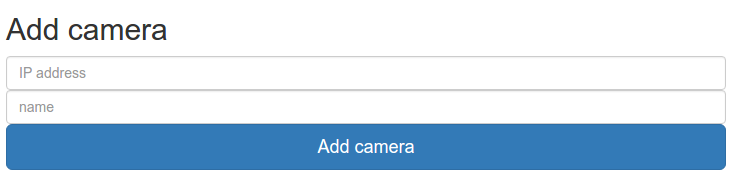
\includegraphics[width=\textwidth]{add_camera_form.png} 
  \caption{Форма добавления камеры} 
  \label{sec:user_guide:add_camera}
\end{figure}

При переходе на главную страницу если у пользователя нет добавленных камер, то его перенаправляет на форму добавления, которую можно увидеть на рисунке \ref{sec:user_guide:add_camera}. На форме добавления камеры у пользователя есть возможность ввести IP адрес камеры и её псевдоним, который и будет передаваться сервису управления шлагбаумами. Сразу при переходе на форму фокус получает поле <<IP address>>, так что пользователь может немедленно начинать вводить сетевой адрес камеры. В случае ошибки пользователю будет показанно всплывающее сообщение об ошибке как показанно на рисунке \ref{sec:user_guide:add_camera_error}, указывающее на поле с ошибкой.

\begin{figure}[ht]
  \centering
  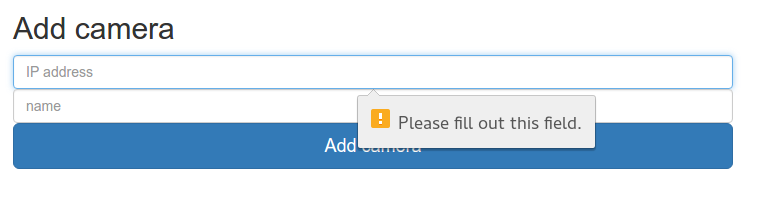
\includegraphics[width=\textwidth]{add_camera_error.png} 
  \caption{Пример ошибки на форме добавления камеры} 
  \label{sec:user_guide:add_camera_error}
\end{figure}

После удачного добавления камеры пользователь будет перенаправлен на главную страницу. На главной странице будут показанны все камеры подключенные к серверу, пример подключенной камеры можно увидеть на изображении \ref{sec:user_guide:main_page_camera}, на которой изображение слева это видеопоток с камеры, под словом <<Address>> находится сетевой адрес подключенной камеры, а под словом <<Name>> приводится псевдоним устройства, на правой части располагаются кнопки управления. 

\begin{figure}[ht]
  \centering
  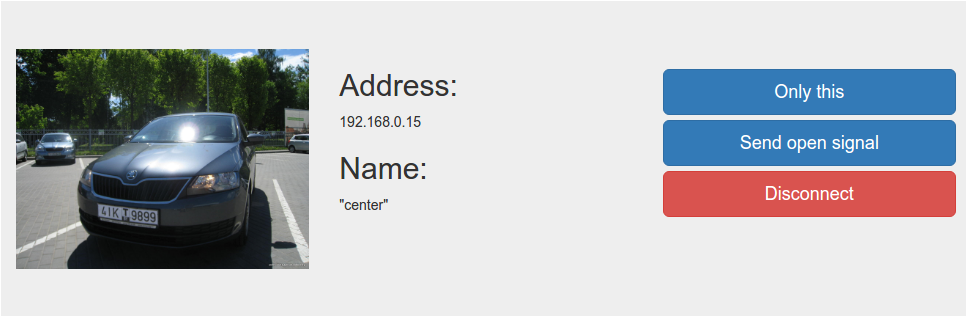
\includegraphics[width=\textwidth]{main_page.png} 
  \caption{Пример подключенной камеры на главной странице} 
  \label{sec:user_guide:main_page_camera}
\end{figure}

При нажатии на кнопку <<Disconnect>> сервер будет отключен от камеры. Заметим что кнопка сделанна красным цветом потому как является опасной, разумеется для безопасности после нажатия на кнопку появится всплывающее окно, изображенное на рисунке \ref{sec:user_guide:danger_action_popup}, которое просит пользователя подтвердить своё намеренье. 

\begin{figure}[ht]
  \centering
  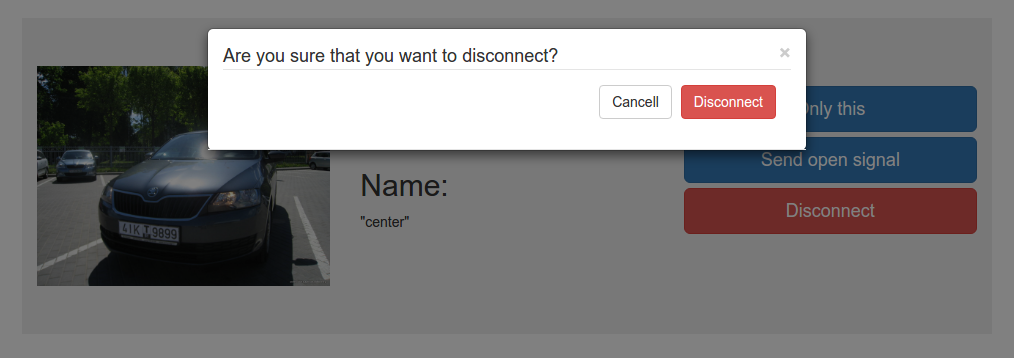
\includegraphics[width=\textwidth]{danger_action_popup.png} 
  \caption{Пример всплывающего окна при выполнении опасного действия} 
  \label{sec:user_guide:danger_action_popup}
\end{figure}

Кнопки <<Send open signal>> сделанна на случай если системе не удается распознать автомобильный номер, но оператору удалось его распознать. Инцидент логируется а сервису шлагбаума отправляется сигнал открытия.

Кнопка <<Only this>> оставляет видеопоток только с этой камеры, как показанно на рисунке \ref{sec:user_guide:only_one_fullscrean}, это удобно когда у персонала есть несколько мониторов и хочется видеть на каждом мониторе свое изображение.

\begin{figure}[ht]
  \centering
  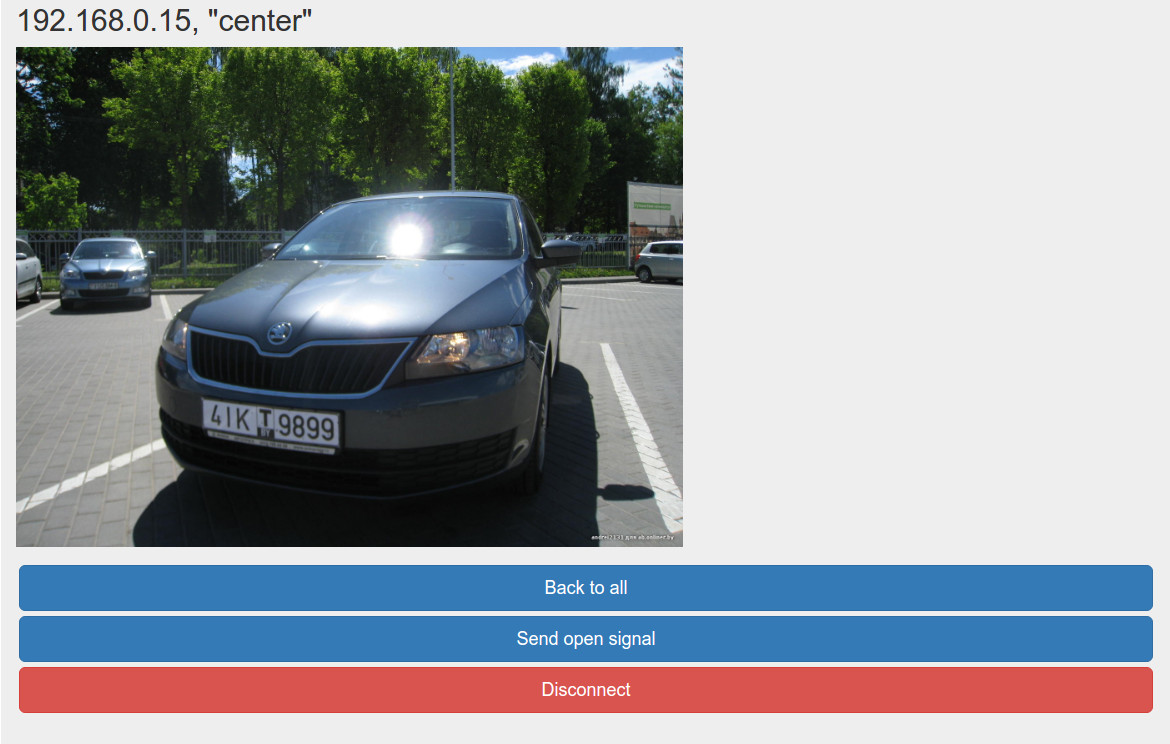
\includegraphics[width=\textwidth]{camera_fullscrean.jpg} 
  \caption{Пример отображения только одной камеры} 
  \label{sec:user_guide:only_one_fullscrean}
\end{figure}

Если пользователь пожелает увидеть подробности о шагах распознавания то на страннице <<Image>> можно загрузить отдельное изображение у увидеть все шаги распознавания как показанно на рисунке \ref{sec:user_guide:log_example}. 

\begin{figure}[ht]
  \centering
  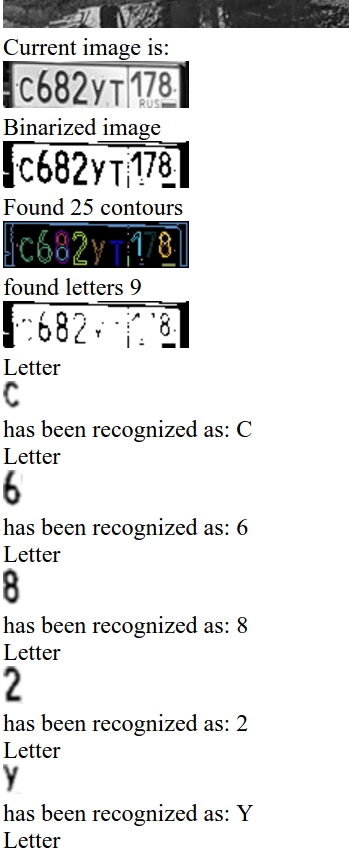
\includegraphics[scale=0.15]{log_example.png} 
  \caption{Пример части страницы всех этапов распознавания} 
  \label{sec:user_guide:log_example}
\end{figure}